% Copyright (C)  2015  Alexander Jankowski, Philipp Hacker.
% Permission is granted to copy, distribute and/or modify this document
% under the terms of the GNU Free Documentation License, Version 1.3
% or any later version published by the Free Software Foundation;
% with no Invariant Sections, no Front-Cover Texts, and no Back-Cover Texts.
% The lincense itself can be found at <https://www.gnu.org/licenses/fdl-1.3>.

\documentclass[numbers=noenddot,a4paper,notitlepage,twoside,BCOR15mm]{scrartcl}
%\documentclass[numbers=noenddot,12pt,a4paper]{scrartcl}

\usepackage{ifoddpage}
\usepackage[infoshow]{tabularx}
\usepackage{fancyhdr}
\usepackage[greek,ngerman]{babel}
\usepackage[T1]{fontenc}
\usepackage[utf8]{inputenc}
\usepackage{libertine}
\usepackage{ziffer}
\usepackage{graphicx}
\usepackage{units}
\usepackage[infoshow]{tabularx}
\usepackage[all]{xy}
\usepackage{amsmath}
\usepackage{amssymb}
\usepackage{wrapfig}
\usepackage{upgreek}
\usepackage{esint}
\usepackage{float}
\usepackage[font=small,labelfont=bf]{caption}
\usepackage{subcaption}
\usepackage{lscape}
\usepackage[backref=page]{hyperref}
\usepackage{cleveref}
\usepackage{csquotes}

\renewcommand{\headrulewidth}{0.1pt}
\renewcommand{\footrulewidth}{0.1pt}
\newcommand{\name}{\text{Philipp Hacker}} %TODO Name des Protokollanten eintragen

\renewcaptionname{ngerman}{\figurename}{Abb. }
\renewcaptionname{ngerman}{\tablename}{Tab.}

\setlength{\parindent}{0pt}

\newcommand{\nummat}[1]{\left[\text{#1}\right]}
\newcommand{\num}[1]{$\left[\text{#1}\right]$}
\newcommand{\degree}{^\circ}
\newcommand{\diff}{\textnormal{d}}
\newcommand{\tenpo}[1]{ 10^{#1}}
\newcommand{\greek}[1]{\greektext#1\latintext}
\newcommand{\ix}[1]{_\text{#1}}
\newcommand{\imag}{\mathbf{i}}
\newcommand{\tilt}[1]{\textit{#1}}
\newcommand{\grad}[1]{\textit{grad}\left(#1\right)}
\newcommand{\divergenz}[1]{\textit{div}\left(#1\right)}
\newcommand{\euler}{\mathnormal{e}}
\newcommand{\fett}[1]{\textbf{#1}}
\newcommand{\einnup}{\hspace{0.2cm}}
\newcommand{\einnum}{\hspace{-0.2cm}}
\newcommand{\zentriert}[1]{\begin{center}#1\end{center}}

\title{Protokoll: Kolloide Plasmen} %TODO Name des Versuchs eintragen
\author{Alexander Jankowski, Philipp Hacker}
\date{\today}
\pagestyle{fancy}
\fancyhead[C]{\thepage}
\fancyhead[R]{\name}
\fancyfoot[C]{\thepage}
\fancyhead[L]{Abschnitt \thesection}

\begin{document}
	\maketitle
	\begin{center}
		Betreuer: Dr. Michael Himpel\\ %TODO Name des Betreuers eintragen
		Versuchsdatum: 16./17.12.2015 \\ %TODO Datum des Versuchs eintragen
		\begin{table}[h]
			\centering
			Note: %TODO Gute Note erhalten :)
			\begin{tabularx}{1.5cm}{|X|}
				\hline \\ \\
				\hline
			\end{tabularx}
		\end{table}
	\end{center}
	\vspace*{\fill}
	\tableofcontents
	\vfill
	\newpage
	\section{Motivation}

		Das Feld der Physik komplexer Plasmen vergrößert sich rasant: nicht nur im Labor, sonder auch bei Experimenten in Schwerelosigkeit oder für Optimierungen der Elektronik-Industrie sind staubige Gasentladungen von großem Interesse. Im Speziellen sind komplexer Plasmen in der Astrophysik sehr wichtig, da sich 99\% des beobachtbaren Volumens im Weltall im Plasma-Zustand befindet. Interstellare Gaswolken, Kometen-Schweife und planetare Ringe wie um Saturn sind alles staubige Plasmen.\\
		Ziel dieses Versuchs soll die präzise Manipulation eines sog. finiten, zweidimensionalen Yukawa-Systems sein. Insbesondere die Untersuchung der Kopplung und die Arbeit mit komplexen Plasmen, sowie der Beobachtungs- und Auswertungsmethodik sollen wichtige Bestandteile dieses Experimentes sein.

		\begin{figure}[!h]
			\centering
			\begin{minipage}{0.49\textwidth}
				\centering
				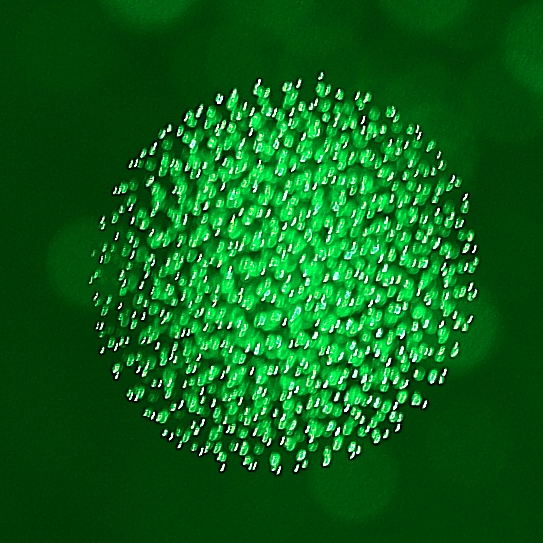
\includegraphics[scale=1.]{figs/cluster.png}
			\end{minipage}
			\begin{minipage}{0.48\textwidth}
				\caption{Mit grünen Nd:YAG-Lasern ausgeleuchteter, dreidimensional ausgedehnter Yukawa-Ball. Der verwendete Staub betsteht aus homogenen, Malamin-Formaldehyd-Kügelchen mit einem Radius im $\upmu$m-Bereich}
			\end{minipage}
		\end{figure}


	\newpage
	\section{Physikalische Grundlagen}

		Der in diesem Versuch genutzte Aufbau entspricht dem eines kapazitiv gekoppelten Niederdruck-Radiofreuquenz-Plasmas.\\
		Befindet sich ein Fremdteilchen, ein Festkörper oder eine weitere Ladungsträgerspezies in so einer Entladung (nicht nur), so spricht man von komplexen Plasmen. Für das Experiment ist dies der Fall, da hierbei in das Plasma homogene Melamin-Formaldehyd-Partikel mit dem Radius $a=\unit[7.1]{\upmu m}$ eingebracht werden. Diese erfahren, in Abhängigkeit der Parameter der Gasentladung, verschiedenste Wechselwirkungen mit den Ladungsträgern und externen Feldern. Inhalt des Experimentes, welches diesem Protkoll zu Grunde liegt, ist die Bestimmung der Staubladung, -temperatur sowie dem mittleren Abstand zwischen den Teilchen einer Schicht.

		\section{Aufladung von Staubpartikeln}\label{sub:ströme}

		Die Ladung eines Fremdteilchens (Staub) in einem Plasma ist eine dynamische Größe. Sie ist sowohl zeitlich veränderlich, als auch abhängig von den Plasmaparametern, den Partikeleigenschaften sowie deren Trajektorie in der Entladung. Die Ladung eines Teilchens zum Zeitpunkt $t$ ergibt sich, näherungsweise, aus den Ladungsströmen $I\ix{k}$ der Plasmaspezies auf das Partikel bis zu diesem Zeitpunkt. Im folgenden genügt es, dieses Problem auf einer Zeitskala zu betrachten, in der man die Ladung als konstant unter dem Einfluss der Ströme annehmen kann. Diese werden damit stationär.

			\begin{align}
				\sum_{\text{k}} I\ix{k}\left(\Phi\ix{fl}\right)=\frac{\diff Q\ix{S}}{\diff t} \,\, . \label{eq:float}
			\end{align}

		Die Elektronen und Ionen im Plasma strömen aufgrund ihrer thermischen Bewegung auf das Fremdteilchen und verleihen diesem über Stöße eine Ladung $Q\ix{S}$, wobei sich für das Partikel ein elektrostatisches Potential $\Phi\ix{fl}$, das sog. \tilt{floating} Potential, einstellt, für welches \autoref{eq:float} die \tilt{Kirchhoff'sche Knotenregel} gilt. Die dominanten Ladungsströme kommen aus dem Plasmas selbst. Hier soll es ausreichen, die Plasmaströme nach \tilt{Langmuir} und \tilt{Mott-Smith} mit dem sog. \tilt{orbital motion limit}-Modell \cite{Langmuir26} zu beschreiben.\\
		Dabei wird angenommen, dass sich ein strömendes Teilchen, welches zu $Q\ix{S}$ beiträgt bzw. damit elektrostatisch wechselwirkt, stoßfrei aus dem Unendlichen (durch die Entladung) darauf zu bewegen kann. Aufgrund der, im Allgemeinen höheren Elektronentemperatur und -beweglichkeit wird $\Phi\ix{fl}<0$, woraus eine veränderte Wechselwirkung mit den Teilchen der Ladungsströme folgt.\\
		Unter der Annahme einer \tilt{maxwell'artigen} Geschwindigkeitsverteilung für Ionen und Elektronen folgen die \autoref{eq:elektronenstrom} und \autoref{eq:ionenstrom}.

			\begin{align}
				\text{Ionen: } I\ix{I}&=\pi a^2n\ix{I}e\sqrt{\frac{8k\ix{B}T\ix{I}}{\pi m\ix{I}}}\left(1-\frac{e\Phi\ix{P}}{k\ix{B}T\ix{I}}\right) \label{eq:ionenstrom} \\
				\text{Elektronen: } I\ix{e}&=-\pi a^2n\ix{e}e\sqrt{\frac{8k\ix{B}T\ix{e}}{\pi m\ix{e}}}\exp\left(\frac{e\Phi\ix{P}}{k\ix{B}T\ix{e}}\right) \label{eq:elektronenstrom}
			\end{align}

		Der Unterschied zwischen \autoref{eq:ionenstrom} und \autoref{eq:elektronenstrom} resultiert aus den unterschiedlichen Arten der Wechselwirkung mit dem Staubteilchen. Da $\Phi\ix{P}<0$ ist, werden Ionen aller Geschwindigkeiten in Richtung des Partikels gelenkt und könnten theoretisch damit stoßen (mit Rücksicht auf die Geschwindigkeitsverteilung und den Streuquerschnitt). Die Elektronen hingegen müssen mindestens eine Geschwindigkeit $v\ix{min}=\sqrt{-2e\Phi\ix{P}/m\ix{e}}$ besitzen, damit sie die Potentialbarriere zum Partikel überwinden und damit stoßen können. Au{\ss}erdem finden sich mit $\sqrt{8k\ix{B}T\ix{j}/\pi m\ix{j}}$ die thermischen Geschwindigkeiten der jeweiligen Spezies $j$ als Vorfaktoren wieder. Damit werden die Gesamtstr\"ome letztendlich zum Produkt aus ungest\"orter, thermischer Stromdichte und der angepassten Wechselwirkungsfl\"ache des Partikels. \\
		Die bezeichneten thermischen Geschwindigkeiten gehen aus der \tilt{Brown'schne Molekularbewegung} hervor. Die genannten Ausdrücke gehen außerdem auf eine \tilt{Maxwell'sche} Geschwindigkeitsverteilung  zurück, wobei diese Herangehensweise (siehe unten) nicht der Realität entspricht.\\
		Es sei erwähnt, dass die OML-Theorie nicht der Realität entspricht. Die mittlere freie Weglänge eines Ions oder Elektrons hat in etwa die Dimension der Debyelänge $\lambda\ix{D}$ und ist nicht, wie vorausgesetzt, unendlich groß. Des weiteren entsprechen die $f\left(v\ix{j}\right)$ in der Praxis nicht isotropen Maxwell-Geschwindigkeitsverteilungen.\\
		Um abschließend die Staubladung zu bestimmen, kann man das Modell eines Kugelkondensators der Kapazität $C\ix{S}$ hernehmen und dieses mit einer Abschirmung $a/\lambda\ix{D}$ verknüpfen (nach \cite{Melzer12}).

			\begin{align}
				Q\ix{S}=Z\ix{S}e=C\ix{S}\Phi\ix{fl}=4\pi\varepsilon\ix{0}a\left(1+\frac{a}{\lambda\ix{D}}\right)\Phi\ix{fl} \label{eq:ladung}
			\end{align}

		Für typische Laborplasmen kann das \tilt{floating}-Potential zu $\Phi\ix{fl}\approx-2k\ix{B}T\ix{e}/e$ genähert werden, woraus die Ladungszahl sich zu $Z\ix{S}\approx1400\cdot a/\unit[1]{\upmu m}\cdot T\ix{e}/\unit[1]{eV}$ ergibt.\\
		In diesem Versuch geht man einen einfacheren, experimentell leichter zugänglichen Weg: die harmonische Anregung einer 2D-Schicht von Staubpartikeln. Dabei wird der sog. \tilt{bias} (Gleichanteil der rf-Spannung, siehe \cite{Piel10}) an der unteren Elektrode - über welcher sich die Schicht Staub im Plasma 'einfängt' - variiert, sodass eine vertikale (z-Richtung) Schwingung des Systems angeregt wird. Es gilt die \autoref{eq:beweg} mit der Neutralgasreibung $\beta$, der Anregung $F\ix{ext}\sin(\omega t)$, der Gravitations- sowie elektrischen Kraft auf das konstant geladene Teilchen $m\ix{S}g$ und $Q\ix{S}E(z)$.

			\begin{align}
				m\ix{S}\ddot{z}+m\ix{S}\beta\dot{z}+Q\ix{S}E(z)-m\ix{S}g+F\ix{ext}\sin(\omega t) \label{eq:beweg}
			\end{align}

		Beachtet man die sog. Ionenwolke um ein jedes Partikel und das in der Randschicht, in welcher die Schicht aus Teilchen eingefangen wird, Elektronenmangel aufweist, so erhält man \cite{Melzer94} aus der Poisson-Gleichung \autoref{eq:efeld}. Verwendet man zusätzlich das Matrix-Schicht-Modell, wonach die Teilchendichten nicht mehr abhängig sind vom Abstand zur Elektrode, so erhält man die allgemein Lösung der reduzierten Bewegungsgleichung zu \autoref{eq:res}.

			\begin{align}
				E\ix{1}(z)=&\frac{e}{\varepsilon\ix{0}}(N\ix{I}(z)n\ix{e}(z)) \label{eq:efeld} \\
				z(t)=&A\ix{0}R(\omega)\sin(\omega t-\varphi(\omega)) \label{eq:res}\\
				R(\omega)=&\left((\omega\ix{0}^2-\omega^2)^2+\beta^2\omega^2\right)^{-1/2} \label{eq:antwort} \\
				\varphi(\omega)=&\frac{\omega\beta}{\omega\ix{0}^2-\omega^2} \\
			\end{align}

		Dabei ist $R(\omega)$ die Resonanzfunktion oder auch Antwortfunktion des vorliegenden Systems. Ein \tilt{fit} dieser Funktion an das Messpektrum ergibt später die Resonanzfrequenz $\omega\ix{0}^2=Q\ix{S}E\ix{1}/m\ix{S}$, womit die Ladung der Partikel bestimmt werden kann.\\
		Für die Berechnung von $Q\ix{S}$ benötigt man jedoch noch die lokale Feldstärke $E\ix{1}$ in der Randschicht. Nach bspw. \cite{Piel10} kann man dafür die \tilt{Bohm-Kriterien} heranziehen. Da diese den Partikeln, welche in die Randschicht eindringen, 'Regeln' bezüglich ihrer Geschwindigkeiten und damit auch Dichten auferlegen, lässt sich näherungsweise $n\ix{I}\approx0,61n\ix{I,0}$ mit $n\ix{I,0}$ der ungestörten Dichte schreiben. Des weiteren kann ein Elektronentastverhältnis in der Randschicht von $\alpha\approx1/3$ angesetzt werden. Das Feld wird letztendlich zu

			\begin{align}
				E\ix{1}=\frac{e}{\varepsilon\ix{0}}0,61n\ix{I,0}(1-\alpha) \,\,. \label{eq:konstfeld}
			\end{align}

	\clearpage

	\subsection{Finite Systeme}

		Ein sog. \tilt{Yukawa-Sytem} kann, wie bereits erwähnt, durch das Erzeugen eines externen Potentials erzeugt werden: beispielsweise durch räumliche Begrenzung mit einer Küvette oder einem Ring, welche sich im Plasma aufladen und damit eine nach innen gerichtete, elektrische Kraft auf den ebenfalls negativ geladenen Cluster ausüben. Das aus den Kräften auf die Staubpartikel resultierende Potential kann als harmonisch angenommen werden, siehe \autoref{img:potential}.In diesem Versuch befindet sich ein Metallring über der unteren Elektrode, welcher den Einfang biete und so die Erzeugung von Yukawa-Sytemen ermöglicht.

			\begin{wrapfigure}{l}{0.47\textwidth}
				\centering
				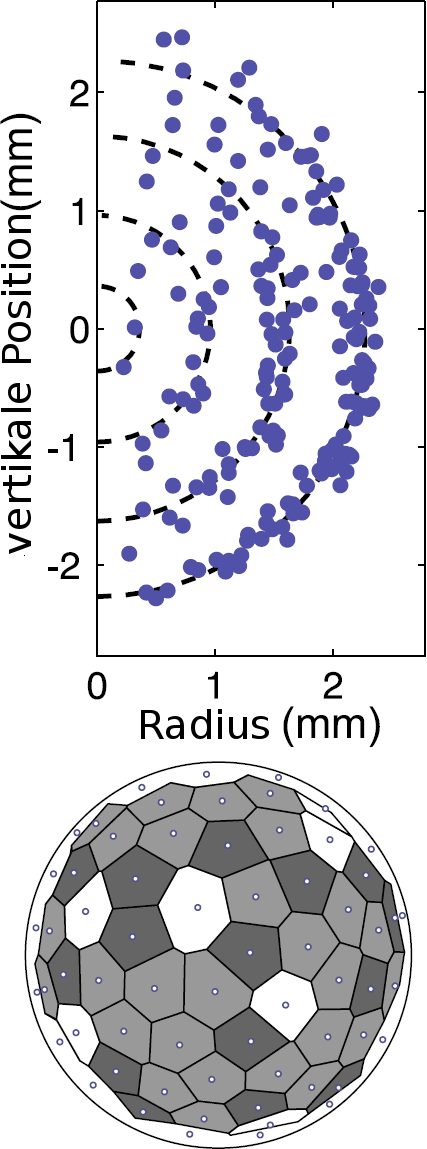
\includegraphics[width=0.32\textwidth,height=0.77\textwidth]{figs/yukawaballN190.png}
				\caption{Teilchen-Verteilung und kristalline Schalenstruktur eines dreidimensional ausgedehnten, sog. \tilt{Yukawa-Balls}, $N=190$ (nach \cite{Arp04})}\label{img:strukturN190}
			\end{wrapfigure}

		Um ein Maß für die Stabilität eines staubigen Plasmas zu erhalten, geht man, wie bei Festkörpern und deren Elektronengasen, von einer Punktladung $Q$ vor dem Hintergrund der Ionen und Elektronen aus (\tilt{one component plasma} - OCP). Der Kopplungsparameter $\Gamma$ in \autoref{eq:kopplung} beschreibt somit die elektrostatische Wechselwirkung eines Teilchens mit seinen Nachbarn in Einheiten der thermischen Energie.\\
		Für ein $\Gamma>1$ spricht man von einer starken Kopplung innerhalb des Clusters bzw. des Plasmas. Mit $\Gamma\geq\Gamma\ix{k}$ liegen kristalline Systeme vor. Bei einem kleineren Wert gehen die Cluster in einen flüssigen bzw. gasförmigen Zustand über (\autoref{img:gamma}). Das heißt, dass ein System aus Staubpartikeln "`schmelzen"' kann, bringt man durch Lasereinstrahlung o.ä. gezielt Energie in den Cluster ein und verringert damit die Ordnung bzw. erhöht die thermische Bewegung. Dabei verschwindet zuerst die Winkelabhängigkeit, was das Auflösen der kristallartigen Strukturen innerhalb des Clusters zur Folge hat.

	\clearpage

			\begin{figure}
				\centering
				\begin{subfigure}[t]{0.48\textwidth}
					\centering
					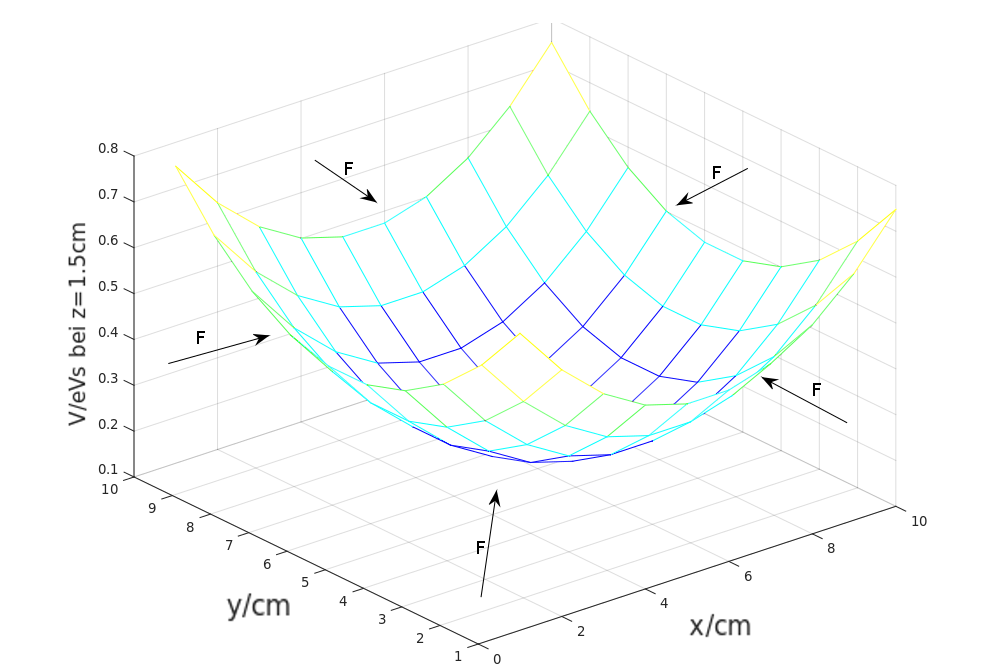
\includegraphics[width=1.1\textwidth,height=0.3\textheight]{figs/einfangpotnu.png}
					\caption{}
					\label{img:potential}
				\end{subfigure}
				\begin{subfigure}[t]{0.48\textwidth}
					\centering
					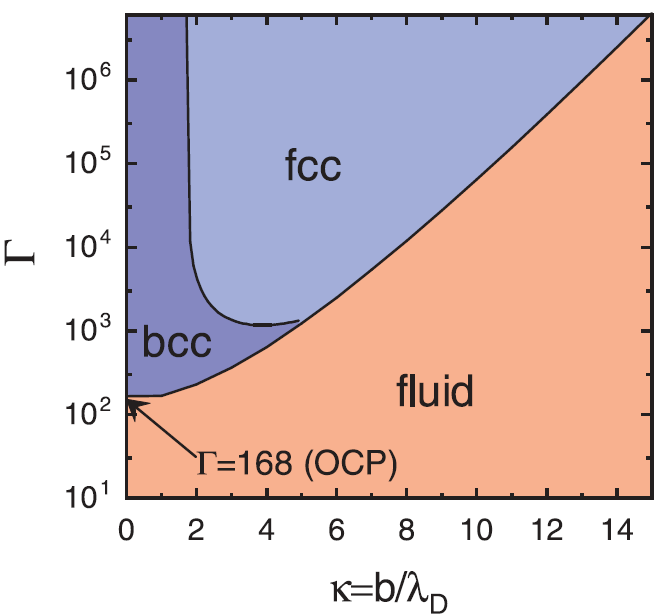
\includegraphics[width=0.9\textwidth,height=0.3\textheight]{figs/gammaphasetransmelzer.png}
					\caption{}
					\label{img:gamma}
				\end{subfigure}
				\caption{\fett{(a)}: Harmonischer Einfang des Potentials $V$ in $\unit{eVs}$ mit globalem Minimum (dunkel). Darstellung für eine Elektrodenhöhe  von $\unit[1,5]{cm}$. \fett{(b)}: Phasendiagramm nach \cite{Melzer12} für eine effektive Coulomb-Kopplung nach \autoref{eq:kopplung}.}
			\end{figure}


			\begin{align}
				\Gamma=\frac{Z\ix{S}e^2}{4\pi\varepsilon\ix{0}b\ix{WS}k\ix{B}T\ix{S}}  \,\,; \quad \Gamma\ix{C,eff}=\Gamma\exp\left(-\frac{b\ix{WS}}{\lambda\ix{D}}\right) \label{eq:kopplung}
			\end{align}

		Die größe $b\ix{WS}$ ist der \tilt{Wigner-Seitz}-Radius: er ist analog zu $\overline{b}$, dem mittleren Teilchenabstand, eine Skala für Längen in diesen Systemen. Insbesondere ist $b\ix{WS}$ eine 'korrektere' Größe, da sich der Staub zweidimensionaler Objekte in hexagonalen bzw. pentagonalen Zellen anordnet. Die Zusammensetzung eines solchen \tilt{finiten Yukawa-Systems} ist in \autoref{img:strukturN190} dargestellt. Außerdem: auf Grund der, auf die Partikel wirkenden Kräfte und der Coulomb-Wechselwirkung des Staubes streben die Systeme bei entsprechenden Umgebungsparametern eine energetisch günstige, kristallartige Struktur an. Der effektive Parameter für Coulomb-Wechselwirkungen $\Gamma\ix{C,eff}$ entspricht einer modifizierten Kopplung mit Rücksicht auf die Abschirmung durch die Ionenwolke (\cite{Lampe00}, \cite{Schweigert00d}) um ein Partikel bzw. den Cluster. Aus diesem Grund führt man die Abschirmstärke $\kappa=b\ix{WS}/\lambda\ix{D}$ ein, welche angibt, um wie viel die elektrostatische Wechselwirkung mit einem Teilchen der Ladung $Q$ innerhalb einer Elementarzelle der Staubpartikel abgeschwächt ist. Außerdem folgt daraus der Zusammenhang für die Phasengrenze in \autoref{img:gamma} $\Gamma\left(\kappa\right)$: für große \tilt{Wigner-Seitz}-Radien bzw. sehr kleine Debye-Längen verschwindet die Wechselwirkung zwischen den Staubteilchen nahezu vollständig.\\
		Nach \cite{WignerRad} kann der Wigner-Seitz-Radius 2-dimensionaler Systeme über \autoref{eq:2dim} abgeschätzt werden.

			\begin{align}
				b\ix{WS}=\left(\frac{\sqrt{3}}{2}\right)^{1/2}\overline{b} \label{eq:2dim}
			\end{align}

	\section{Durchführung}

		Wie bereits erwähnt handelte es sich bei diesem Versuch um ein kapazitiv gekoppeltes, Niederdruck-rf-Plasma. Die Elektrodenfrequenz lag typischerweise bei $\unit[13,56]{MHz}$. Die Kammer ist prinzipiell wie ein Plattenkondensator konzipiert: eine untere, scheibenförmige Elektrode liegt direkt an dem rf-Generator mit einige Watt Leistung an, der übrige Teil der Kammer ist geerdet. Somit liegt eine asymmetrische Entladung vor, was insbesondere Konsequenzen für die Ausbildung der Randschicht und den \tilt{bias} hat. \"Uber eine Pumpe wird die Kammer bis auf einen Restdruck von etwa $\unit[\tenpo{-1}]{Pa}$ evakuiert, damit sie m\"oglichst frei von Umgebungsluft ist und anschlie{\ss}end eine Argon-Entladung bei $\unit[5-15]{Pa}$ erzeugt werden kann.
		Weiterhin befindet sich im Deckel der Kammer eine Durchf\"uhrungen f\"ur den Staub aus MF (Melamin-Formaldehy) - $\unit[7,1]{\upmu m}$ im Radius  mit einer Dichte von $\unit[1514]{kg/m^3}$. Die Partikel werden \"uber ein Reservoir der Gr\"o{\ss}e eines 1 Cent-St\"uckes mit einer $\unit{\upmu m}$-gro{\ss}en Bohrung in die Entladung eingebracht.\\
		Zur Verfügung steht außerdem eine Laserdiode mit $\lambda=\unit[685]{nm}$ und einer maximalen Leistung von $\unit[1]{W}$. Dazu befinden sich eine Zylinderlinse zur Auffächerung des Strahls zwischen Kammer und Laser.\\
		Die Kammer hat einen Innendurchmesser von $\approx\unit[20]{cm}$, wobei deren Deckel und Boden aus Edelstahl und die Wände aus Aluminium bestehen. Vier gro{\ss}e, seitlich angebrachte Fenster erm\"oglichen,  aus der Ebene den Blick auf das Experiment. Im Deckel der Kammer befindet sich ein weiteres, kreisrundes Fenster. Die Beobachtung des Systems wird durch zwei zueinander orthogonal CCD-Kameras realisiert, wobei diese durch die genannten Glas-Einsätze in der Kammer schauen.

		\paragraph{Versuchstag 1, 16.12.2015}

			Nach Inbetriebnahme des Aufbaus - Argon einfüllen, Druck auf $\unit[14,9]{pa}$ regeln, rf-Generator einschalten und eine eingespeiste Leistung von $\unit[7]{W}$ einstellen - galt es, eine möglichst zweidimensionale Struktur aus Staubpartikeln einzufangen. Dies gestaltete sich durchaus als kompliziert, da bereits viele Teilchen im Reservoir durch die Umgebungsluft oder Prozesse im Plasma verklumpt waren und diese Störkörper das zu betrachtende System manipulierten. Wiederholtes ein- und ausschalten des Plasmas, und damit das 'Auswerfen' der Partikel, wurde genutzt, um letztendlich eine Schicht aus ca. 13 Teilchen zu erzeugen.\\
			Dieser Einrichtung schloss sich die externe Anregung des Elektrodenbias und somit des Systems über einen Frequenzgenerator an. Bei festgehaltener Amplitude wurde die Frequenz im Bereich zwischen $\unit[4,997]{Hz}$ und $\unit[31]{Hz}$ variiert, um eine grobe Abschätzung des Resonanzverhaltens zu bekommen. Danach wurden Aufnahmen für feste Frequenzen über 100 frames (in 4 Sekunden, 25 fps) mit der Seitenkamera gemacht. Dafür wurde die Kamera auf das Experiment bestmöglich fokussiert. Die Blende wurde so eingestellt, dass der Hintergrund dunkel, die Teilchen jedoch noch gut sichtbar waren. Man erhielt schließlich ein Bildersequenz im *.bmp-Format in Graustufen.

		\paragraph{Versuchstag 2, 17.12.2015}

			Im Vorfeld des zweiten Versuchstages wurde der Staub im Reservoir erneuert, sodass Verklumpungen nicht mehr den Einfang erschwerten.\\
			Nach erneuter Inbetriebnahme (gleiches Verfahren) bei $\unit[14,6]{pa}$ Arbeitsgas-Druck und $\unit[7]{W}$ \fett{IN} sowie $\unit[1]{W}$ \fett{OUT} wurde erneut ein 2D-System mit rund 21 Teilchen erzeugt. Dabei verfuhr man wie am ersten Tag. Um Informationen über die mittleren Teilchenabstände sowie Verschiebungen pro Zeit - auf Grund der Brown-Bewegung - wurde mit der Oberkamera eine Aufnahme über 1000 frames bei 60 frames pro Sekunde gemacht. Die Einstellung der CCD-Kamera wurden analog zum ersten Versuch unternommen. Man erhielt gleichartige Daten.\\
			Nach dieser Messung schaltete man das Experiment ab, schloss alle Ventile und ließ wieder Umgebungsluft in die Kammer, um diese zu Öffnen. An die Stelle, an welcher das System eingefangen wurde, galt es dann, ein Stück Millimeterpapier zu platzieren. Dieses nutzte man dann für die Kalibration bezüglich der Ortsauflösung bei \underline{unverändertem} Fokus der Kamera.

				\begin{figure}[H]
					\centering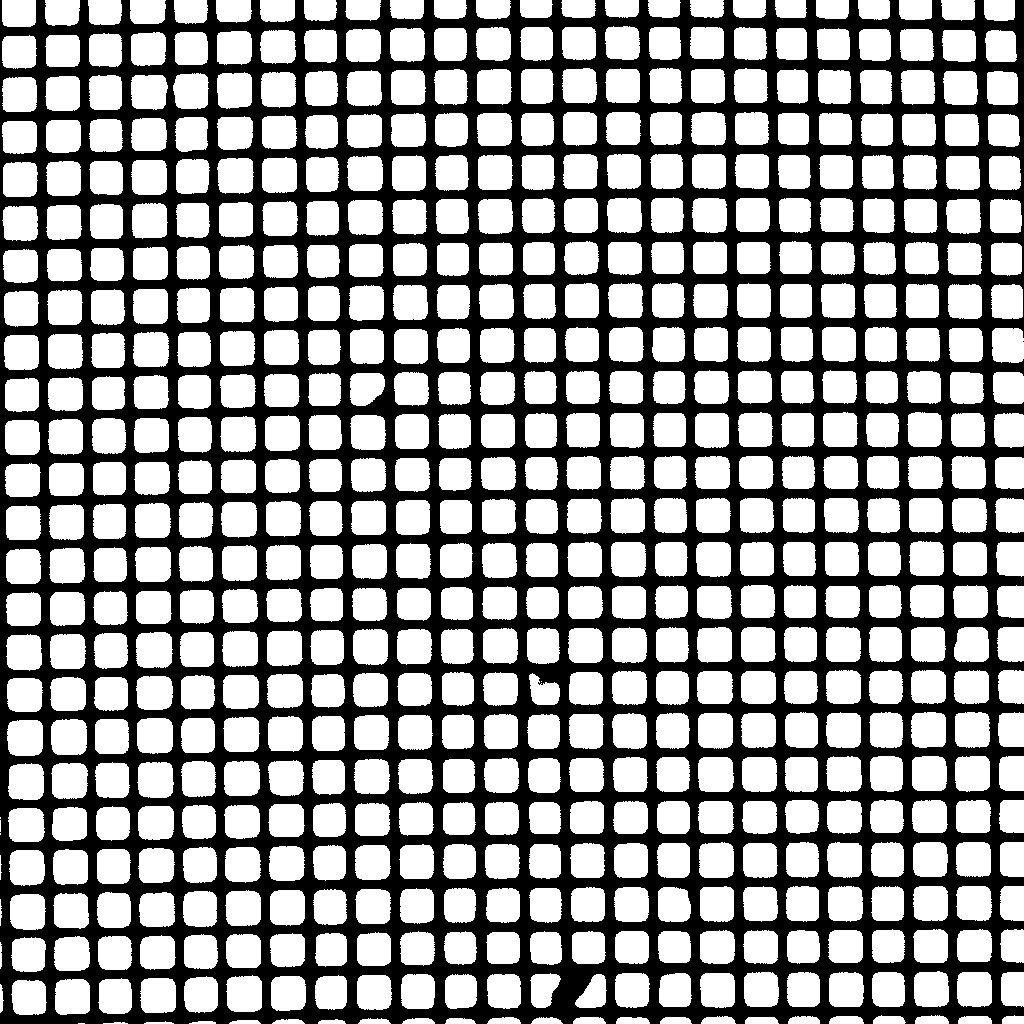
\includegraphics[width=0.5\textwidth]{figs/0-1.png}
					\caption{Kalibration mit Millimeterpapier.}\label{img:milli}
				\end{figure}

	\newpage
	\section{Auswertung}

	\vspace{-1cm}
		\begin{figure}[H]
			\begin{minipage}{0.45\textwidth}

			\subsection{Bestimmung der Staubladung}
				Nach Erhalt der Bilddateien wurden die Sequenzen aus den *.bmp-Bildern für jeweils eine Anregungsfrequenz überlagert. Mit Hilfe von Benutzer-Abfragen in einer graphischen Oberfläche  (\tilt{ginput(n)}) wurden dann die maximalen Auslenkungen der Teilchen in vertikaler Richtung bestimmt. Man erhielt eine Art überbelichtetes Bild über die gesamte Messdauer. Die \autoref{tab:ladu} zeigt die Werte in Pixeln zu den Anregungsfrequenzen. Zusammen mit einem Fit der Antwortfunktion \autoref{eq:res} zeigt \autoref{img:freq} das graphische Ergebnis.

			\end{minipage}
			\hspace{1cm}
			\begin{minipage}{0.3\textwidth}
				\centering
				\begin{table}[H]
					\begin{tabular}{c|c}
						\hline Frequenz in Hz & normierte Amplitude \\ 
						\hline \hline 4,997 & 0,083 \\
						\hline 7,022 &  0,153\\ 
						\hline 9,033 &  0,16\\ 
						\hline  10,93&  0,191\\ 
						\hline  13,05&  0,247\\ 
						\hline  15,05&  0,312\\ 
						\hline  17,04&  0,425\\ 
						\hline  18,04&  0,599,\\ 
						\hline 19,04 &  0,912\\ 
						\hline  20,04&  1\\ 
						\hline  21,04&  0,801\\ 
						\hline  22,03&  0,598\\ 
						\hline  23,02&  0,4\\ 
						\hline  25,01&  0,268\\ 
						\hline  27,0&  0,206\\ 
						\hline  29,11&  0,181\\ 
						\hline  31,0& 0,125 
					\end{tabular}
					\caption{Frequenze und normierte Amplituden der Aufnahme von Versuchstag 1.}\label{tab:ladu}
				\end{table}

			\end{minipage}
		\end{figure}

		\begin{figure}[H]
			\centering
			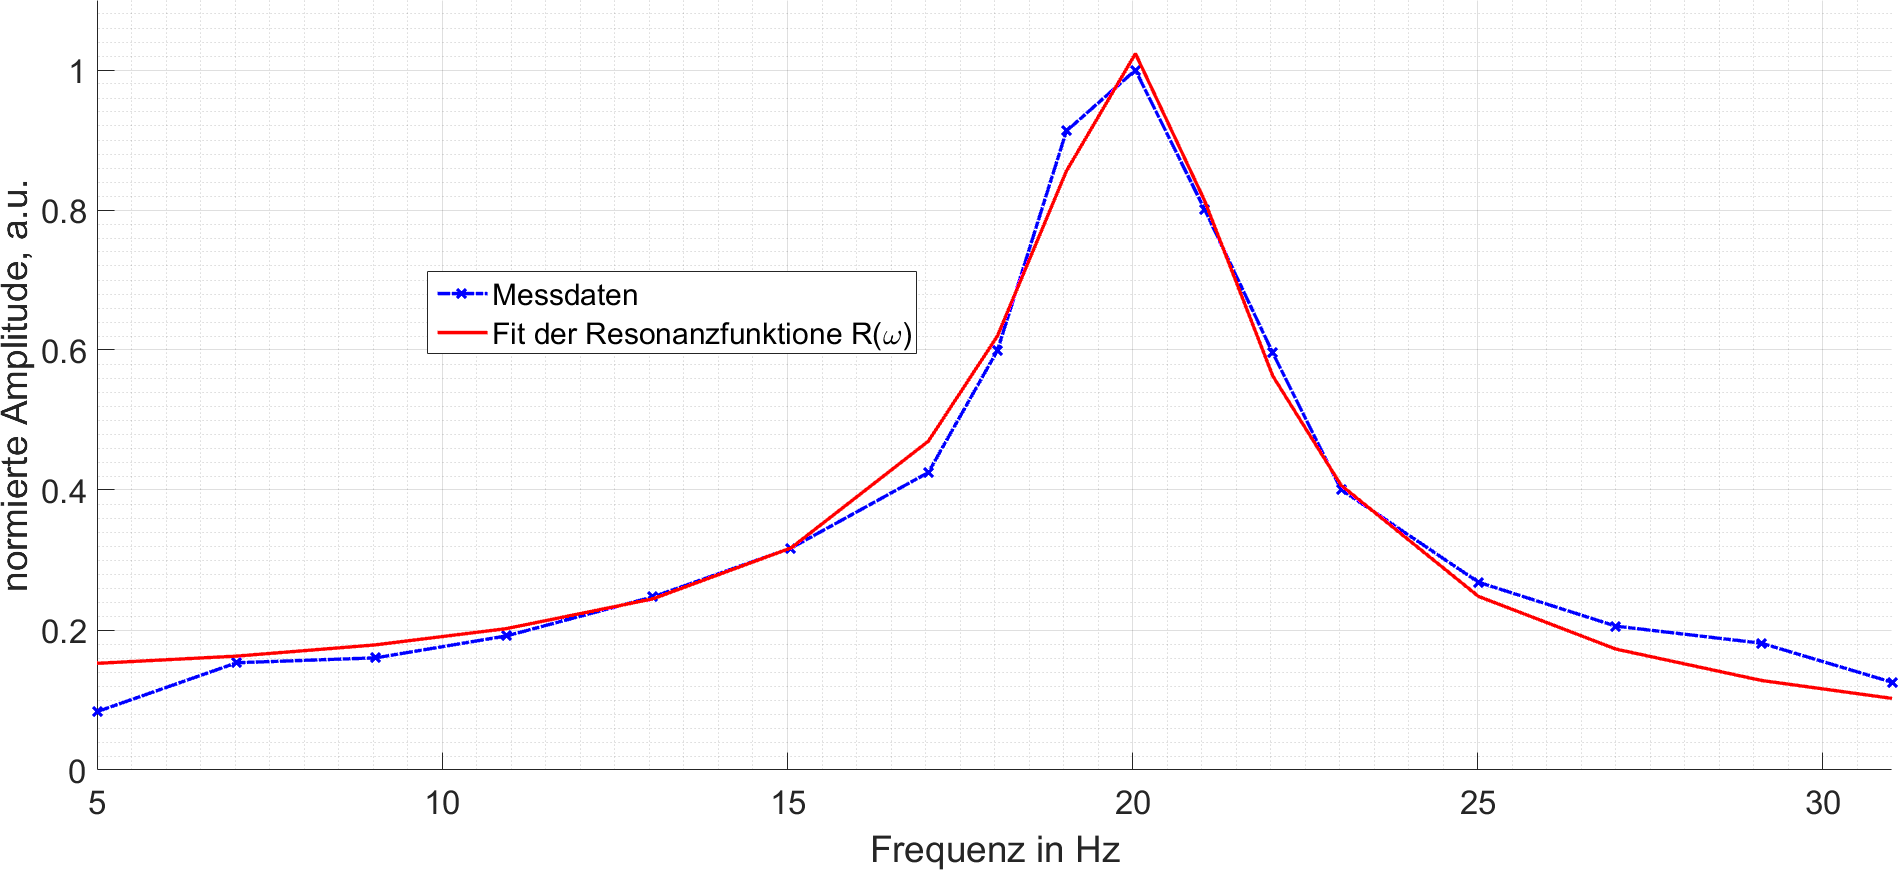
\includegraphics[width=\textwidth]{figs/res_schick.png}
			\caption{Resonanzantwort der 2D-Schicht von Teilchen bei externer Anregung über den Elektroden-bias. Fit der Resonanzfunktion \autoref{eq:res}.}\label{img:freq}
		\end{figure}

	\clearpage

		Der Reibungskoeffizient wurde zu $\beta=\unit[17,682]{1/s}$.	Die Resonanzfrequenz bzw. die Kreis-Resonanzfrequenz ergab sich als:

			\begin{align}
				f\ix{0}=\unit[20,088]{Hz} \quad \omega\ix{0}=\unit[126,22]{rad/s} \,\, .\label{eq:resfreq}
			\end{align}

		Mit der gegebene Dichte, dem Radius und $m\ix{S}=4/3\pi a^3\rho$ ergibt sich eine Masse zu $\unit[2,269\tenpo{-12}]{kg}$ je Teilchen. Bei einer Leistung von $\unit[7]{W}$ und einem Druck von $\approx\unit[15]{pa}$ erhält man aus \cite{EMAUGreifswaldPlasm} eine Elektronendichte im Plasma von $\approx\unit[0.7\tenpo{15}]{m^{-3}}$. Über \autoref{eq:konstfeld} und $n\ix{e}=\alpha n\ix{I}$ folgt damit eine Feldstärke in der Randschicht über der Elektrode von $\unit[4,152\tenpo{7}]{V/m}$.\\
		Über die Definition der Resonanzfrequenz $\omega\ix{0}^2=Q\ix{S}E\ix{1}/m\ix{s}$ ergibt sich letztendlich

			\begin{align}
				Q\ix{S}=\unit[8,71\tenpo{-16}]{Coul}\approx 5436\cdot e \label{eq:lad}
			\end{align}

	\subsection{Thermische Geschwindigkeit}

		Mit Hilfe der zur Verfügung gestellten Software \tilt{KristallAuswertung.m} wurde die mittlere Verschiebung der Teilchen von einem frame zum anderen in den Aufnahmen des 2. Versuchstages bestimmt. Wichtig dabei ist, dass nur 9 der ca. 21 Teilchen im System von der Software betrachtet wurden. Es wurde mit rund 60 fps für 1000 frames aufgenommen. \\
		Das Programm ermittelte eine Verschiebung von $\unit[0,99\pm 0.68]{px}$ pro Bild. Da der Fehler die Größenordnung des Ergebnisses hat, ist dieses Ergebnis zu hinterfragen.\\
		Mittels der Kalibration mit dem Millimeterpapier (siehe \autoref{img:milli}) erhielt man den Maßstab von $\unit[43,01]{px/mm}$. Damit wird die mittlere thermische Geschwindigkeit zu

			\begin{align}
				v\ix{th,S}=\unit[0,023]{mm/frame}=\unit[1,381]{mm/s} \,\, .\label{eq:geschw}
			\end{align}

		Zusammen mit dem, von der Software angegeben Fehler erhält man, dass der Wahre Wert $v\ix{th,true}$ im Intervall $\left[2,329; 0,4324\right]\unit{mm/s}$ liegen muss. Das Unterstreicht die Aussage von vorher wiederum, da die Intervalllänge etwa die Dimension des ersten Wertes hat.\\
		Im gleichen Zuge wie die Festlegung der Skalen, kann die Bestimmung des mittleren Teilchenabstandes $\overline{b}$ vorgenommen werden. Man erhält den Wert $\unit[0,795]{mm}$, woraus sich der Wigner-Seitz-Radius nach \autoref{eq:2dim} zu

			\begin{align}
				b\ix{WS}=\unit[0,739]{mm} \label{eq:wigner}
			\end{align}

		ergibt.\\
		Somit kennen wir alle wichtigen Größen des Systems. Damit können wir weitere Berechnungen anstellen: nach $v\ix{th,S}^2=8k\ix{B}T\ix{S}/(\pi m\ix{S})$ (analog \autoref{eq:elektronenstrom} usw.) bestimmt man die Staubtemperatur.

			\begin{align}
				T\ix{S}=\unit[123174]{K}\,\hat{=}\,\unit[10,61]{eV} \label{eq:temp}
			\end{align}

	\subsection{Kopplungsparameter und Fehlerbetrachtung}

		Da alle notwendigen Größen für die Berechnung von \autoref{eq:kopplung} nun bekannt sind, errechnet man leicht dessen Wert. Zusätzlich ist in \cite{EMAUGreifswaldPlasm} die Debye-Länge $\lambda\ix{D}=(525\pm25)\unit{\upmu m}$ gegeben.

			\begin{align}
				\Gamma=5,423\quad\Gamma\ix{C,eff}=1,326 \label{eq:koppwert}
			\end{align}

		Das spricht offensichtlich für ein stark gekoppeltes System, in welchem aber noch die thermische und elektrische Wechselwirkung die gleichen Dimensionen besitzen. Auch in Rückblick auf die Ladung bzw.die Ladungszahl scheinen die erhaltenen Größen realistisch. In derartigen Laborplasmen sind $\tenpo{2}\dots\tenpo{4}\cdot e$ gegeben. Auch die thermische Energie von $\approx\unit[10]{eV}$ ist im Rahmen der Experiment-Parameter eine gute Größe.\\
		Wählt man eine andere Herangehensweise an die Staubladung, nämlich über \autoref{eq:ladung}, so ergeben sich gänzlich andere Größen. Des Weiteren ist die Elektronendichte aus \cite{EMAUGreifswaldPlasm} bekannt, weswegen die dafür notwendige Elektronentemperatur bestimmt werden kann ($\approx0,61n\ix{e,0}$). Bezieht man außerdem noch das Fehlerintervall der Debye-Länge mit ein, so ergeben sich die folgenden Größen:

			\begin{align}
				T\ix{e}\in&\left[\unit[27130]{K}; \unit[22421]{K}\right] \nonumber\\
				Z\ix{S}\in&\left[23346; 19319\right] \nonumber\\
				\Gamma\in&\left[100,03; 68,5\right] \nonumber\\
				\Gamma\ix{C,eff}\in&\left[26,08; 15,61\right]\,\,. \nonumber
			\end{align}

		Im Hinblick auf die Kopplungsparameter und Staubtemperaturen erscheinen diese Ergebnisse sinnvoller, als die obigen. Der Wert von $\Gamma$ deutet eine sehr starke, aber noch keine kristalline Kopplung an. Der Effektiv-Wert repräsentiert das ebenfalls. Die Beobachtungen am System - schwache Amplituden, kleines thermisches Schwanken - stimmen mehr mit den neuen Größenintervallen überein, als die vorherigen. Das Modell des gedämpften, getriebenen harmonischen Oszillators als Staubteilchen kann also als ungenügend betrachtet werden.\\
		Für die benutzerdefinierte Eingaben kann man einen Fehler von $\pm\unit[2]{px}$ ansetzen.Die Abweichungen pflanzen sich folgendermaßen fort:

			\begin{align}
				b\ix{WS}\in&\left[\unit[0.781]{mm}; \unit[0.698]{mm}\right] \nonumber \\
				Z\ix{S}\in&\left[5831; 5012\right] \nonumber \\
				T\ix{S}\in&\left[\unit[9,68]{eV}; \unit[11,67]{eV}\right] \nonumber \\
				v\ix{th,S}\in&\left[\unit[1,319]{mm/s}; \unit[1,448]{mm/s}\right] \nonumber \\
				\Gamma\in&\left[5,624; 5,253\right] \nonumber \,\,.
			\end{align}

		Die Auswirkungen der Fehler in einer GUI sind allgemein gering. Sie verändern die Interpretationsmöglichkeiten der errechneten Werte nicht.\\
		Abschließend bleibt die Frage, ob und in welcher Ordnung ein Fehler in der Ermittlung von $\overline{b}$ und dem mittleren Schwankungsquadrat in \tilt{KristallAuswertung.m} vorliegt.

	\newpage
	\section{Anhang}

		\bibliography{all.bib}
		\bibliographystyle{unsrt}

\end{document}